\subsection{\secState{R}Weather Impact}\label{sec:WeatherImpact}

\paragraph{Idea:} The \emph{climate} has stable properties throughout the year. There are observations that climate is shifting in Europe, the periods of sprint/autumn weather are shortening, the periods of summer and winter are prolonging. 

Overall the \emph{European Climate} is getting similar to \emph{North America`s} continental climate. This has a severe impact on many aspects of modern society including transportation, especially aviation, emerging UAS industry. 

The key fact is that the occurrence of critical weather conditions, like storms or heavy winds is increasing. Along with the increasing intensity of these events, the magnitude increases to non-construction mitigable levels.

\paragraph{Transportation Impact:} The \emph{train transportation} is the most robust and very infrastructure dependant transportation type. On the other hand, the \emph{aerial transportation} infrastructure is sparse, and most of the maneuvering is done in open airspace. 

\emph{Weather Impact} on transportation, in general, has been introduced by Koetse in the study \cite{koetse2009impact}. The \emph{bad weather} situations are well avoidable by \emph{general aviation}. The \emph{general aviation} avoidance capability comes from the \emph{high organization} of controlled \emph{airspace}, high grade of surveillance equipment (weather radar).

The situation with \emph{UAS} systems is different; they usually have more delicate construction and significantly smaller takeoff weight. The \emph{weather} could be even harsher on the lower altitudes. The \emph{implementation} of \emph{weather avoidance} is necessary for \emph{safe UAS operations} in non-controlled airspace. The \emph{UAS operations} can stick to existing weather avoidance approaches in controlled airspace. 

The \emph{challenge} to avoid weather situations is similar to the geo-fencing problem on low altitudes. The \emph{serious weather case} can be encapsulated into a protected area with some \emph{altitude limitations}.

\paragraph{Weather avoidance:} \emph{Weather-based} preemptive planning was introduced into manned aviation in 2015 \cite{yamashita2015climate}. There is a  global approach to weather avoidance. Meaning there is one global \emph{weather model}. Similar impact on every \emph{controlled airspace} attendant. This impact model needs to be refined for various \emph{aircraft classes}.  

\begin{note}
    The \emph{UAS classes} are summarized in (tab. \ref{tab:smallDroneClessesAccordingtoEASA}), the \emph{separation minima} is specified in (tab. \ref{tab:proposedseparationMinimaforUAS}). This needs to be accounted in weather impact calculation. 
    
    The \emph{separation minima} are also accounted for \emph{weather} separation. The \emph{UAS} must keep minimal distance to \emph{dangerous weather condition}.
    
    The radius and impact zone of \emph{dangerous weather condition} is evaluated concerning \emph{UAS} class; the 5 kg machine is more impacted than 150 kg machine or \emph{autonomous personal transportation}.
\end{note}
    
\emph{Severe Weather Condition Detection Capabilities} for the current level of standard aviation equipment have been reviewed in \cite{smith2016multi}. The capability is sufficient for medium scale \emph{UAS} (25 kg). The \emph{numeric models} for \emph{local airspace cluster} can have precision up to one cubic meter of air. The precision of \emph{numeric prediction} depends on \emph{weather stations} density and equipment precision.

The \emph{dynamic} routing of \emph{aircraft} (manned aviation) has been outlined in Balaban et al. \cite{balaban2017dynamic}. The operational space is separated into \emph{altitude layers} where each layer is separated into homogeneous euclidean grid cells. Each cell (fig. \ref{fig:localizedWeatherModelExample}) has an evaluation of \emph{relative humidity} (fig. \ref{fig:humidityRelativeLocalizedExample}), \emph{temperature}, \emph{wind velocity and heading} (fig.\ref{fig:localizedWindVectorsExample}). There is possible to make a prediction and route all aircraft in advance. The scaling challenge also remains for this approach. 

\begin{figure}[H]
	\centering
	\begin{subfigure}{0.45\textwidth}
		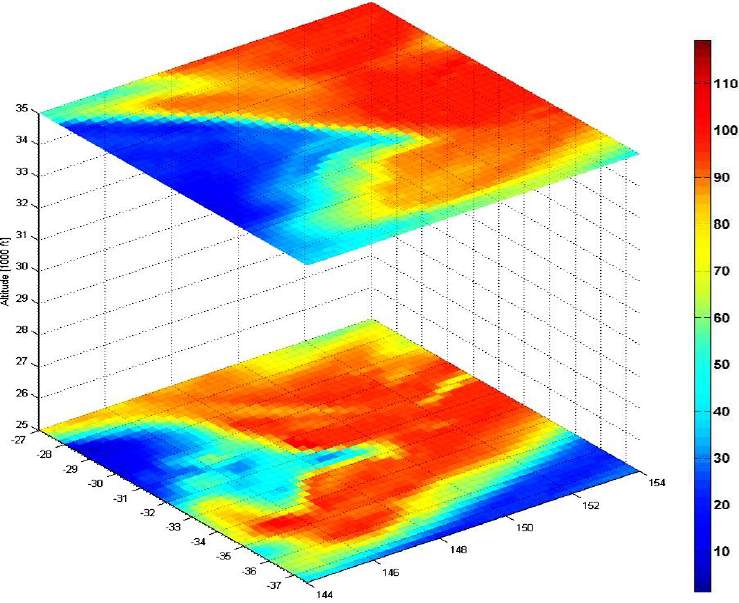
\includegraphics[width=\textwidth]{\FIGDIR/02_03_RelativeHumidity}
		\caption{Relative Humidity.} 
		\label{fig:humidityRelativeLocalizedExample}
	\end{subfigure}
	\vspace{1em} 
	\begin{subfigure}{0.45\textwidth} % width of right subfigure
		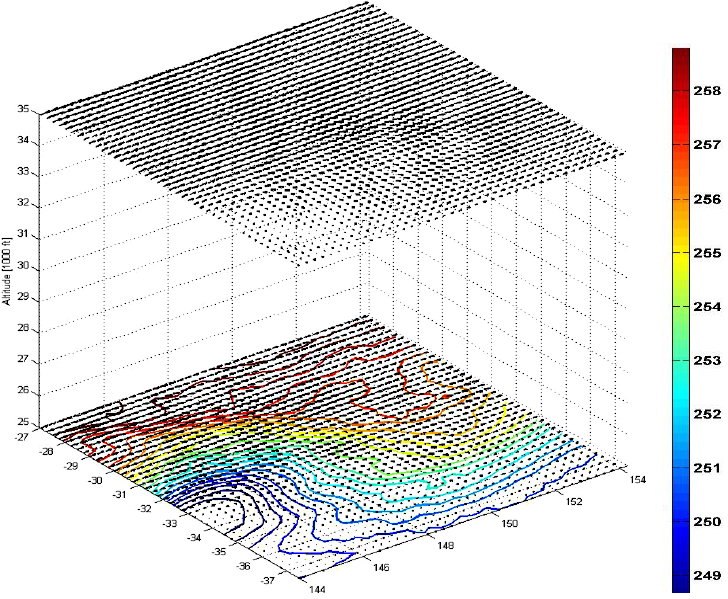
\includegraphics[width=\textwidth]{\FIGDIR/02_04_WindTemperature}
		\caption{Localized Wind Vectors.} % subcaption
		\label{fig:localizedWindVectorsExample}
	\end{subfigure}
	\caption{Localized Weather Model \cite{balaban2017dynamic}.} % caption for whole figure
	\label{fig:localizedWeatherModelExample}
\end{figure}
    
\paragraph{Localized Weather Impact Example:} An \emph{Icing Risk} in a localized environment have been predicted based on the numerical model \cite{thompson2017numerical}. It is shown that icing can be prevented by \emph{planned} and \emph{reactive} avoidance. The prevention can be done by placing hard or soft constraint into an environment. 

    
\paragraph{Weather Models:} \emph{Weather Models} can be extracted from \emph{Climate and weather model archive at the National Oceanic and Atmospheric Administration} \cite{rutledge2006nomads}. There is an example of troposphere winds (0 - 60 000 feet AMSL) (fig. \ref{fig:ExampleOfTroposphereWinds}) which can be useful in fuel-efficient route planning. 
    
\begin{figure}[H]
    \centering
    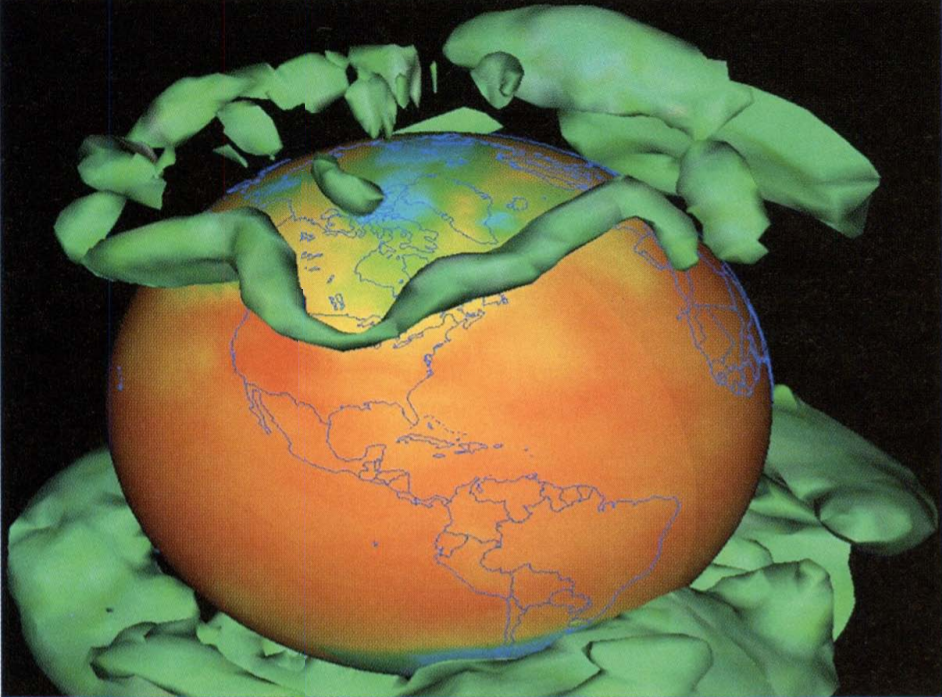
\includegraphics[width=0.7\textwidth]{\FIGDIR/02_01_IVS_Model}
    \caption{Example of upper troposphere winds \cite{rutledge2006nomads}.}
    \label{fig:ExampleOfTroposphereWinds}
\end{figure}